\chapter{Perambatan Sinyal: Gelombang Berjalan dan Gelombang Berdiri}\label{ch:b1:wave-propagation}

Petiklah senar gitar dan seluruh aula mendengar sebuah nada; sentuhlah
titik tengahnya dengan jari dan nadanya melompat satu oktaf. Berdirilah
di antara dua pengeras suara yang membunyikan nada yang sama dan, sambil
berjalan perlahan, Anda melewati bintik-bintik yang nyaris senyap setiap
beberapa desimeter. Cahaya dari dua lubang jarum melukis garis-garis
pada layar. Tak ada apa pun yang terbawa dari satu tempat ke tempat lain
dalam peristiwa itu --- tak ada udara, tak ada senar, tak ada kaca yang
berpindah --- namun ada yang merambat: sebuah \emph{\omterm{def:b1:wave-propagation:signal}{sinyal}}. Bab ini
menggambarkan bagaimana \omterm{def:b1:wave-propagation:signal}{sinyal} bergerak, apa itu gelombang sinusoidal,
dan apa yang terjadi ketika dua gelombang bertemu: matematika
superposisi, interferensi, dan \omterm{thm:b1:wave-propagation:standing}{gelombang berdiri}, yang akan dipakai
kembali oleh setiap bab gelombang berikutnya --- akustika, optika, dan
fisika kuantum.

\begin{omfigure}
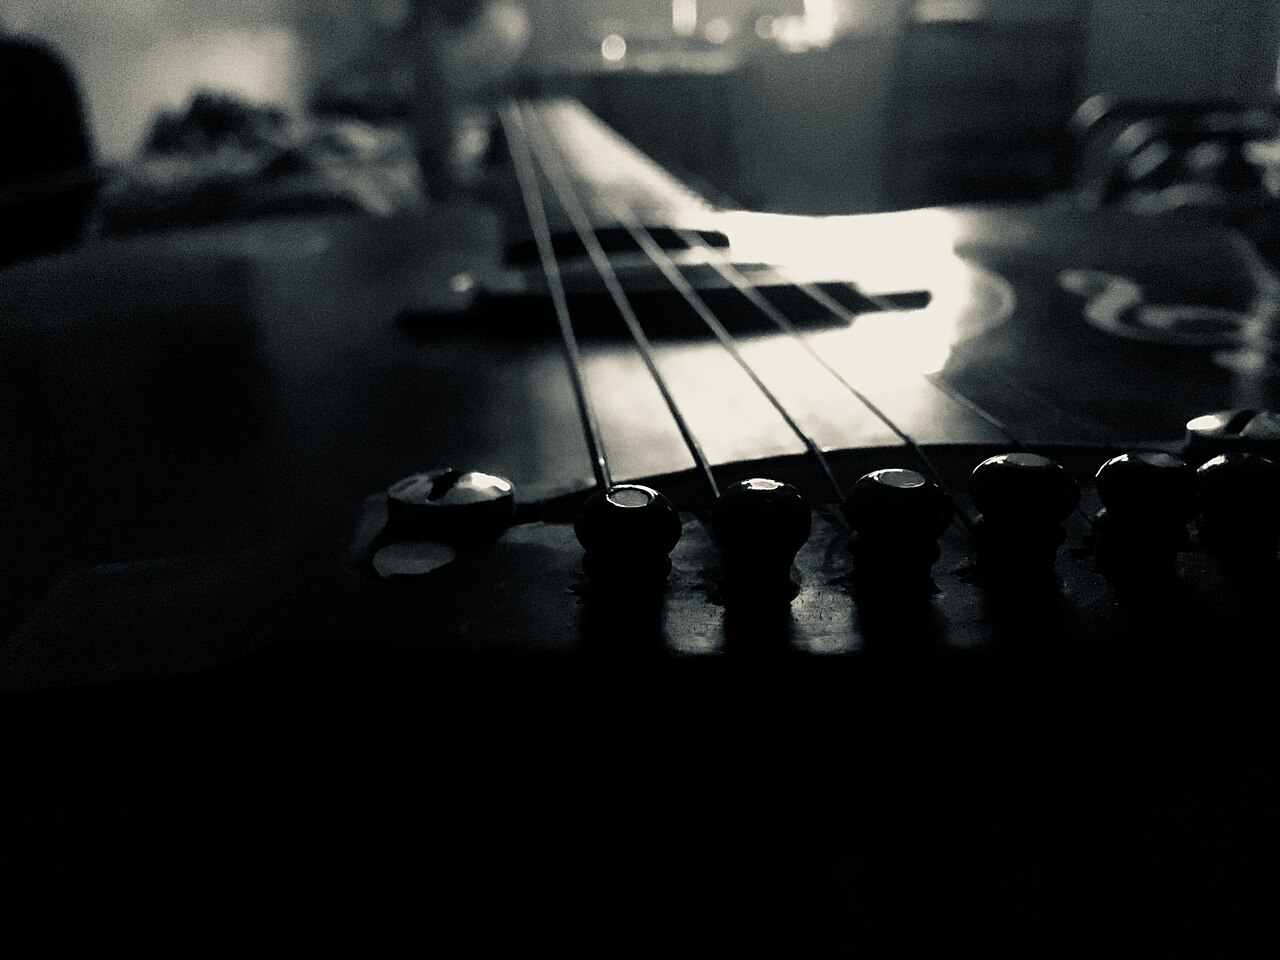
\includegraphics[width=0.55\linewidth]{images/book3/guitar-closeup.jpg}

{\small Enam senar, enam \omterm{prop:b1:wave-propagation:modes}{frekuensi dasar}: masing-masing adalah \omterm{thm:b1:wave-propagation:standing}{gelombang berdiri} yang terpasak di nat dan di jembatannya, dan jari memendekkannya untuk meninggikan nadanya.}
\end{omfigure}

\section{Sinyal}

\begin{definition}[Sinyal; sinyal sinusoidal]\label{def:b1:wave-propagation:signal}
\index{sinyal}\index{sinyal sinusoidal}\index{amplitudo}\index{fase}\index{frekuensi sudut}
Sebuah \emph{sinyal} adalah \omterm{def:b1:units-dimensions:unit}{besaran fisis} yang berubah terhadap waktu
dan membawa informasi: tekanan lebih akustik pada sebuah mikrofon,
tegangan pada sebuah antena, simpangan melintang sebuah titik senar.
\emph{Sinyal sinusoidal}
\[
s(t) = A\cos(\omega t + \varphi)
\]
mempunyai \emph{amplitudo} $A > 0$, \emph{frekuensi sudut} $\omega$
(\unit{rad/s}), \emph{frekuensi} $f = \omega/2\pi$, \emph{periode}
$T = 1/f$ dan \emph{fase awal} $\varphi$; $\omega t + \varphi$ adalah
\emph{fase}nya pada saat $t$.
\end{definition}

\begin{remark}[Spektrum]\label{rem:b1:wave-propagation:spectrum}
\index{spektrum!sinyal}\index{harmonik}
Setiap \omterm{def:b1:wave-propagation:signal}{sinyal} berkala berperiode $T$ adalah jumlah sinusoid berfrekuensi
$f_1 = 1/T$ (\emph{nada dasar}) dan kelipatannya $nf_1$
(\emph{harmonik}); daftar \omterm{def:b1:wave-propagation:signal}{amplitudonya} adalah \emph{spektrum} \omterm{def:b1:wave-propagation:signal}{sinyalnya}.
Seruling dan biola yang membunyikan nada yang sama berbagi nada dasarnya
dan berbeda spektrumnya --- itulah warna bunyi. Penguraiannya (menurut
Fourier) dinyatakan dan dipakai dalam
\cref{ch:b1:filters-transfer-functions}; di sini ia penting karena
sinusoid merambat secara sederhana, dan apa pun yang berlaku bagi tiap
sinusoid berlaku pula, lewat penjumlahan, bagi \omterm{def:b1:wave-propagation:signal}{sinyal} apa pun.
\end{remark}

\begin{proposition}[Layangan]\label{prop:b1:wave-propagation:beats}
\index{layangan}
Jumlah dua sinusoid beramplitudo sama dan berfrekuensi berdekatan
$f_1 > f_2$,
\[
A\cos(2\pi f_1 t) + A\cos(2\pi f_2 t)
= 2A\cos\!\big(2\pi\tfrac{f_1 - f_2}{2}\,t\big)\cos\!\big(2\pi\tfrac{f_1 + f_2}{2}\,t\big),
\]
adalah sinusoid pada frekuensi rata-ratanya yang \omterm{def:b1:wave-propagation:signal}{amplitudonya}
$\abs{2A\cos(\pi(f_1 - f_2)t)}$ membengkak dan memudar pada
\emph{frekuensi layangan} $f_1 - f_2$.
\end{proposition}

\begin{proof}
$\cos a + \cos b = 2\cos\frac{a - b}{2}\cos\frac{a + b}{2}$. Faktor
lambatnya lenyap dua kali tiap periodenya sendiri $2/(f_1 - f_2)$,
sehingga selubung $\abs{\cdot}$ berfrekuensi $f_1 - f_2$.
\end{proof}

\begin{omfigure}
\begin{tikzpicture}
\begin{axis}[omaxis, axis x line=bottom, width=11.5cm, height=4.6cm, xlabel={$t$ (\unit{s})},
    ylabel={$s$}, xmin=0, xmax=1, ymin=-2.3, ymax=2.3, ytick={-2,0,2},
    yticklabels={$-2A$,$0$,$2A$}, xtick={0,0.25,0.5,0.75,1}]
  \addplot[omDef, thick, domain=0:1, samples=700] {cos(deg(2*pi*22*x)) + cos(deg(2*pi*20*x))};
  \addplot[omThm, thick, dashed, domain=0:1, samples=200] {2*cos(deg(2*pi*1*x))};
  \addplot[omThm, thick, dashed, domain=0:1, samples=200] {-2*cos(deg(2*pi*1*x))};
\end{axis}
\end{tikzpicture}

{\small Layangan antara \qty{22}{Hz} dan \qty{20}{Hz}: osilasi
\qty{21}{Hz} yang selubungnya (garis putus-putus) melayang dua kali tiap
sekon --- selisih kedua frekuensinya.}
\end{omfigure}

\begin{example}[Melaras dengan telinga]\label{ex:b1:wave-propagation:tuning}
Garpu tala \qty{440}{Hz} dan senar \qty{443}{Hz} yang dibunyikan
bersama berdenyut tiga kali tiap sekon; mengencangkan senarnya
memperlambat denyutnya, dan ketika denyutnya berhenti senarnya sudah
laras. Telinga mendengar frekuensi rata-ratanya (\qty{441.5}{Hz})
sebagai tinggi nadanya dan selubung \qty{3}{Hz}-nya sebagai kenyaringan
yang bergoyang: layangan membuat selisih frekuensi kurang dari satu
persen menjadi terdengar.
\end{example}

\section{Gelombang berjalan}

\begin{definition}[Gelombang berjalan, cepat rambat]\label{def:b1:wave-propagation:travelling}
\index{gelombang berjalan}\index{cepat rambat}\index{medium tak dispersif}
\omterm{def:b1:wave-propagation:signal}{Sinyal} $s(x, t)$ yang terdefinisi sepanjang sebuah sumbu disebut
\emph{gelombang berjalan} yang bergerak ke arah $+x$ dengan
\emph{cepat rambat} $c$ jika
\[
s(x, t) = f\!\left(t - \frac{x}{c}\right) = F(x - ct)
\]
untuk suatu fungsi $f$ (atau $F$): bentuknya terbawa tanpa berubah,
tergeser sejauh $c\,\Delta t$ dalam waktu $\Delta t$. Gelombang yang
bergerak menuju $-x$ berbentuk $g(t + x/c)$. Medium yang di dalamnya
setiap bentuk merambat tanpa cacat dengan $c$ yang sama disebut
\emph{tak dispersif}.
\end{definition}

\begin{proposition}[Tundaan]\label{prop:b1:wave-propagation:delay}
\omterm{def:b1:wave-propagation:signal}{Sinyal} yang diterima di $x_2$ adalah \omterm{def:b1:wave-propagation:signal}{sinyal} yang dipancarkan di
$x_1 < x_2$, tertunda sebesar $\tau = (x_2 - x_1)/c$:
$s(x_2, t) = s(x_1, t - \tau)$.
\end{proposition}

\begin{proof}
$s(x_2, t) = f(t - x_2/c) = f\big((t - \tau) - x_1/c\big) = s(x_1, t - \tau)$.
\end{proof}

\begin{example}[Cepat rambat]\label{ex:b1:wave-propagation:celerities}
Bunyi di udara, \qty{340}{m/s}: guruh \qty{3}{s} setelah kilatnya
menempatkan sambarannya \qty{1}{km} jauhnya. Bunyi di air,
\qty{1500}{m/s}; di baja, \qty{5000}{m/s}. Gelombang melintang pada
senar bertegangan $F$ dan bermassa tiap satuan panjang $\mu$:
$c = \sqrt{F/\mu}$, seperti diramalkan analisis dimensi
(\cref{exo:b1:units-dimensions:5}) --- \qty{140}{m/s} untuk senar gitar.
Cahaya di hampa, $c = \qty{3.00e8}{m/s}$; di kaca, $c/n$. \omterm{def:b1:wave-propagation:travelling}{Cepat
rambatnya} adalah sifat mediumnya, bukan sifat sumbernya: bisikan dan
teriakan tiba bersama.
\end{example}

\begin{proposition}[Gelombang berjalan sinusoidal]\label{prop:b1:wave-propagation:sinusoidal}
\index{panjang gelombang}\index{bilangan gelombang}\index{kecepatan fase}\index{keberkalaan ganda}
Sumber sinusoidal $s(0, t) = A\cos(\omega t)$ melepaskan
\[
s(x, t) = A\cos\!\big(\omega(t - x/c)\big) = A\cos(\omega t - kx),
\qquad k = \frac{\omega}{c} = \frac{2\pi}{\lambda},
\qquad \lambda = cT = \frac{c}{f}.
\]
Gelombangnya berkala dalam waktu (berperiode $T$) dan dalam ruang
(berperiode \emph{panjang gelombang} $\lambda$); $k$ adalah
\emph{\omterm{prop:b1:wave-propagation:sinusoidal}{bilangan gelombang}}; dua titik yang berjarak $d$ berosilasi dengan
beda \omterm{def:b1:wave-propagation:signal}{fase} $\Delta\varphi = 2\pi d/\lambda = kd$ --- sefase jika
$d = n\lambda$, berlawanan \omterm{def:b1:wave-propagation:signal}{fase} jika $d = (n + \tfrac12)\lambda$. Laju
gerak sebuah puncak, $v_\varphi = \omega/k$, disebut \emph{\omterm{prop:b1:wave-propagation:sinusoidal}{kecepatan
fase}}; di sini $v_\varphi = c$.
\end{proposition}

\begin{proof}
Substitusikan $f(u) = A\cos(\omega u)$ ke dalam $f(t - x/c)$. Pada $x$
tetap \omterm{def:b1:wave-propagation:signal}{sinyalnya} berulang setelah $T = 2\pi/\omega$; pada $t$ tetap ia
berulang setelah $\lambda$ dengan $k\lambda = 2\pi$. Dua titik $x_1$,
$x_2 = x_1 + d$: \omterm{def:b1:wave-propagation:signal}{fasenya} berselisih $kd$. Sebuah puncak
($\omega t - kx = \text{tetap}$) bergerak dengan $\dd x/\dd t = \omega/k$.
\end{proof}

\begin{omfigure}
\begin{tikzpicture}
\begin{axis}[omaxis, width=7.2cm, height=4.2cm, xlabel={$x$}, ylabel={$s(x, t_0)$},
    xmin=0, xmax=6.5, ymin=-1.4, ymax=1.6, ytick={-1,0,1}, yticklabels={$-A$,$0$,$A$},
    xtick={0,2,4,6}, xticklabels={$0$,$\lambda$,$2\lambda$,$3\lambda$}]
  \addplot[omDef, thick, domain=0:6.5, samples=200] {cos(deg(pi*x))};
  \draw[Stealth-Stealth, omThm] (axis cs:2,1.2) -- (axis cs:4,1.2) node[midway, above, font=\footnotesize] {$\lambda$};
  \draw[-Stealth, omExo, thick] (axis cs:4.7,1.2) -- (axis cs:5.7,1.2) node[midway, above, font=\footnotesize] {$c$};
\end{axis}
\end{tikzpicture}\qquad
\begin{tikzpicture}
\begin{axis}[omaxis, width=7.2cm, height=4.2cm, xlabel={$t$}, ylabel={$s(x_0, t)$},
    xmin=0, xmax=6.5, ymin=-1.4, ymax=1.6, ytick={-1,0,1}, yticklabels={$-A$,$0$,$A$},
    xtick={0,2,4,6}, xticklabels={$0$,$T$,$2T$,$3T$}]
  \addplot[omDef, thick, domain=0:6.5, samples=200] {cos(deg(pi*x))};
  \draw[Stealth-Stealth, omThm] (axis cs:2,1.2) -- (axis cs:4,1.2) node[midway, above, font=\footnotesize] {$T$};
\end{axis}
\end{tikzpicture}

{\small \omterm{prop:b1:wave-propagation:sinusoidal}{Keberkalaan ganda} sebuah \omterm{def:b1:wave-propagation:travelling}{gelombang berjalan} sinusoidal: potret
pada waktu tetap berulang setiap panjang gelombang $\lambda$ dan meluncur
dengan laju $c$; \omterm{def:b1:wave-propagation:signal}{sinyal} pada sebuah titik tetap berulang setiap periode
$T$, dengan $\lambda = cT$.}
\end{omfigure}

\begin{definition}[Dispersi]\label{def:b1:wave-propagation:dispersion}
\index{medium dispersif}
Sebuah medium disebut \emph{dispersif} bila \omterm{prop:b1:wave-propagation:sinusoidal}{kecepatan fasenya} bergantung
pada frekuensinya. \omterm{def:b1:wave-propagation:signal}{Sinyal} tak sinusoidal, yang merupakan jumlah
sinusoid, lalu berubah bentuk sambil berjalan, karena komponennya saling
menjauh. Bunyi di udara dan cahaya di hampa bersifat tak dispersif;
cahaya di kaca (\cref{ch:b1:rays-reflection-refraction}) dan gelombang
di air dalam bersifat dispersif --- alun panjang dari badai yang jauh
tiba sehari sebelum riak pendeknya.
\end{definition}

\section{Superposisi dan interferensi}

\begin{theorem}[Superposisi]\label{thm:b1:wave-propagation:superposition}
\index{asas superposisi}
Dalam medium linear, ketika beberapa gelombang merambat bersama, \omterm{def:b1:wave-propagation:signal}{sinyal}
hasilnya pada tiap titik dan tiap saat adalah jumlah \omterm{def:b1:wave-propagation:signal}{sinyal} yang akan
dihasilkan tiap gelombang sendirian.
\end{theorem}
\admitted

\begin{remark}[Kelinearan]\label{rem:b1:wave-propagation:linearity}
Superposisi adalah pernyataan tentang persamaan mediumnya (yang linear
terhadap \omterm{def:b1:wave-propagation:signal}{sinyalnya}), yang benar selama \omterm{def:b1:wave-propagation:signal}{amplitudonya} tetap kecil: bunyi
di bawah ambang nyeri, cahaya di bawah intensitas pemotong laser, senar
yang dipetik lembut. Dua berkas cahaya bersilangan tanpa saling
mengganggu; dua riak saling menembus lalu keluar utuh. Apa yang teramati
\emph{di tempat keduanya bertindih} adalah pokok bahasan interferensi.
\end{remark}

\begin{theorem}[Dua sinyal sinusoidal berfrekuensi sama]\label{thm:b1:wave-propagation:fresnel}
\index{interferensi}\index{rumus Fresnel}\index{interferensi konstruktif}\index{interferensi destruktif}
Pada sebuah titik tempat dua \omterm{def:b1:wave-propagation:signal}{sinyal sinusoidal} berfrekuensi sama tiba,
$s_1 = A_1\cos(\omega t + \varphi_1)$ dan $s_2 = A_2\cos(\omega t + \varphi_2)$,
jumlahnya adalah sinusoid berfrekuensi sama yang \omterm{def:b1:wave-propagation:signal}{amplitudonya} memenuhi
\[
A^2 = A_1^2 + A_2^2 + 2A_1A_2\cos\Delta\varphi,
\qquad \Delta\varphi = \varphi_2 - \varphi_1 .
\]
Untuk gelombang yang intensitasnya (daya tiap satuan luas) sebanding
dengan $A^2$, intensitasnya menuruti \emph{rumus Fresnel}
\[
I = I_1 + I_2 + 2\sqrt{I_1 I_2}\,\cos\Delta\varphi .
\]
Interferensinya \emph{konstruktif} ($A = A_1 + A_2$) ketika
$\Delta\varphi = 2n\pi$, dan \emph{destruktif} ($A = \abs{A_1 - A_2}$)
ketika $\Delta\varphi = (2n + 1)\pi$, $n \in \Z$.
\end{theorem}

\begin{proof}
Jabarkan: $s_1 + s_2 = (A_1\cos\varphi_1 + A_2\cos\varphi_2)\cos\omega t -
(A_1\sin\varphi_1 + A_2\sin\varphi_2)\sin\omega t = X\cos\omega t -
Y\sin\omega t = A\cos(\omega t + \varphi)$ dengan $A^2 = X^2 + Y^2 =
A_1^2 + A_2^2 + 2A_1A_2(\cos\varphi_1\cos\varphi_2 + \sin\varphi_1\sin\varphi_2)$.
Secara geometri: $A$ adalah panjang jumlah dua vektor yang panjangnya
$A_1$, $A_2$ dan membentuk sudut $\Delta\varphi$ (aturan kosinus).
\end{proof}

\begin{proposition}[Dua sumber sefase; beda lintasan]\label{prop:b1:wave-propagation:pathdiff}
\index{beda lintasan}
Dua sumber yang memancar sefase pada panjang gelombang $\lambda$, pada
jarak $d_1$ dan $d_2$ dari sebuah titik $M$, tiba di $M$ dengan
$\Delta\varphi = 2\pi\,\delta/\lambda$, dengan $\delta = d_2 - d_1$
sebagai \emph{\omterm{prop:b1:wave-propagation:pathdiff}{beda lintasan}}nya. Interferensi di $M$ konstruktif jika
$\delta = n\lambda$, dan destruktif jika $\delta = (n + \tfrac12)\lambda$.
\end{proposition}

\begin{proof}
Tiap gelombang tiba dengan ketertinggalan \omterm{def:b1:wave-propagation:signal}{fase} $kd_i = 2\pi d_i/\lambda$
akibat perjalanannya (\cref{prop:b1:wave-propagation:sinusoidal});
selisihnya $2\pi(d_2 - d_1)/\lambda$. Terapkan
\cref{thm:b1:wave-propagation:fresnel}.
\end{proof}

\begin{example}[Dua pengeras suara]\label{ex:b1:wave-propagation:speakers}
Dua pengeras suara yang berjarak \qty{2.0}{m} membunyikan nada
\qty{850}{Hz} yang sama secara sefase ($\lambda = \qty{0.40}{m}$). Pada
sumbu bagi tegaknya $\delta = 0$: keras di mana-mana. Sepanjang ruas
yang menghubungkan keduanya, $\delta$ berubah sebesar $2\lambda$ tiap
panjang gelombang perpindahan, sehingga bintik senyapnya
($\delta = \pm\lambda/2, \pm 3\lambda/2, \dots$) duduk setiap
$\lambda/2 = \qty{20}{cm}$ --- sebuah \omterm{thm:b1:wave-propagation:standing}{gelombang berdiri}, pokok bahasan
subbab berikutnya. Baliklah kabel salah satu pengerasnya sehingga ia
berbunyi berlawanan \omterm{def:b1:wave-propagation:signal}{fase}, dan yang keras dan yang senyap bertukar tempat.
\end{example}

\begin{example}[Lubang Young]\label{ex:b1:wave-propagation:young}
\index{lubang Young}\index{jarak antarpita}\index{lintasan optik}
Dua lubang jarum $S_1$, $S_2$ yang berjarak $a$, disinari satu sumber
ekawarna (sehingga keduanya memancar sefase), mengirimkan cahaya ke
layar berjarak $D \gg a$. Pada sebuah titik layar yang berketinggian $x$
dari sumbunya, \omterm{prop:b1:wave-propagation:pathdiff}{beda lintasannya}
\[
\delta = S_2M - S_1M \approx \frac{a\,x}{D}
\]
(untuk $x \ll D$: $S_{1,2}M = \sqrt{D^2 + (x \mp a/2)^2} \approx D +
(x \mp a/2)^2/2D$, lalu kurangkan). Pita terang pada $x = n\lambda D/a$:
\emph{\omterm{ex:b1:wave-propagation:young}{jarak antarpita}}nya adalah
\[
i = \frac{\lambda D}{a} .
\]
Dengan $a = \qty{0.50}{mm}$, $D = \qty{2.0}{m}$, $\lambda = \qty{633}{nm}$:
$i = \qty{2.5}{mm}$ --- sebatang mistar mengukur panjang gelombang
cahaya. Di dalam medium berindeks $n$, \omterm{prop:b1:wave-propagation:pathdiff}{beda lintasan} yang harus dipakai
adalah \emph{\omterm{ex:b1:wave-propagation:young}{lintasan optik}}, yaitu $n \times$ panjangnya, karena
$\lambda = \lambda_0/n$.
\end{example}

\begin{omfigure}
\begin{tikzpicture}[font=\small, x=1cm, y=1cm]
  \fill (0,0.4) circle (1.5pt) node[left] {$S_1$};
  \fill (0,-0.4) circle (1.5pt) node[left] {$S_2$};
  \draw[Stealth-Stealth] (-0.9,0.4) -- (-0.9,-0.4) node[midway, left] {$a$};
  \draw[thick] (5.6,-2.2) -- (5.6,2.2); \node[above] at (5.6,2.2) {layar};
  \fill[omThm] (5.6,1.3) circle (1.5pt) node[right] {$M$};
  \draw[omDef] (0,0.4) -- (5.6,1.3); \draw[omDef] (0,-0.4) -- (5.6,1.3);
  \draw[dashed] (0,0) -- (5.6,0) node[below right] {$O$};
  \draw[Stealth-Stealth] (5.9,0) -- (5.9,1.3) node[midway, right] {$x$};
  \draw[Stealth-Stealth] (0,-2.0) -- (5.6,-2.0) node[midway, below] {$D$};
  \node[omDef] at (2.8,1.2) {$d_1$}; \node[omDef] at (3.3,0.28) {$d_2$};
  % fringes pattern
  \begin{scope}[xshift=7.6cm]
  \begin{axis}[omaxis, axis x line=bottom, width=4.2cm, height=5.2cm, xlabel={$I$}, ylabel={$x$},
      xmin=0, xmax=4.6, ymin=-2.2, ymax=2.2, xtick={0,4}, xticklabels={$0$,$4I_0$},
      ytick={-2,-1,0,1,2}, yticklabels={$-2i$,$-i$,$0$,$i$,$2i$}, anchor=origin, at={(0,0)}]
    \addplot[omThm, thick, domain=-2.2:2.2, samples=300] ({4*cos(deg(pi*x))^2},{x});
  \end{axis}
  \end{scope}
\end{tikzpicture}

{\small \omterm{ex:b1:wave-propagation:young}{Lubang Young}: dua sumber sefase yang berjarak $a$ mencapai titik
$M$ sebuah layar jauh menyusuri lintasan yang berselisih
$\delta \approx ax/D$. Intensitas pada layarnya, $4I_0\cos^2(\pi x/i)$,
berselang-seling terang dan gelap dengan \omterm{ex:b1:wave-propagation:young}{jarak antarpita} $i = \lambda D/a$.}
\end{omfigure}

\begin{remark}[Koherensi]\label{rem:b1:wave-propagation:coherence}
\index{koherensi}
Rumus Fresnel mengandaikan beda \omterm{def:b1:wave-propagation:signal}{fase} yang tetap. Dua lampu yang terpisah
mempunyai \omterm{def:b1:wave-propagation:signal}{fase} yang melompat secara acak miliaran kali tiap sekon;
rata-rata $\cos\Delta\varphi$ menjadi nol dan intensitasnya sekadar
bertambah: tak ada pita. Interferensi menuntut sumber yang
\emph{koheren} --- dalam praktiknya, dua gelombang yang keluar dari satu
sumber, lewat dua lubang, dua celah, dua muka selaput tipis, atau sebuah
pembelah berkas. Dua pengeras suara yang digerakkan satu pembangkit
bersifat koheren; dua penyanyi tidak.
\end{remark}

\section{Gelombang berdiri}

\begin{theorem}[Gelombang berdiri]\label{thm:b1:wave-propagation:standing}
\index{gelombang berdiri}\index{simpul}\index{perut}
Dua gelombang sinusoidal beramplitudo dan berfrekuensi sama yang
berjalan berlawanan arah berjumlah
\[
A\cos(\omega t - kx) + A\cos(\omega t + kx) = 2A\cos(kx)\cos(\omega t),
\]
sebuah \emph{\omterm{thm:b1:wave-propagation:standing}{gelombang berdiri}}: setiap titik berosilasi sefase (atau
berlawanan \omterm{def:b1:wave-propagation:signal}{fase}) dengan \omterm{def:b1:wave-propagation:signal}{amplitudo} $2A\abs{\cos kx}$ yang bergantung pada
kedudukannya --- nol di \emph{simpul} $x = (n + \tfrac12)\lambda/2$, dan
maksimum di \emph{perut} $x = n\lambda/2$; simpulnya berjarak
$\lambda/2$. Tak ada yang merambat: variabel $x$ dan $t$ terpisah.
\end{theorem}

\begin{proof}
$\cos a + \cos b = 2\cos\frac{a - b}{2}\cos\frac{a + b}{2}$ dengan
$a = \omega t - kx$, $b = \omega t + kx$.
\end{proof}

\begin{proposition}[Moda senar yang terikat kedua ujungnya]\label{prop:b1:wave-propagation:modes}
\index{moda}\index{frekuensi dasar}\index{percobaan Melde}
Senar sepanjang $L$, bercepat rambat $c$, yang terikat di $x = 0$ dan
$x = L$, hanya dapat menopang \omterm{thm:b1:wave-propagation:standing}{gelombang berdiri} sinusoidal jika $L$
merupakan bilangan bulat setengah panjang gelombang:
\[
\lambda_n = \frac{2L}{n}, \qquad f_n = n\,\frac{c}{2L} = n f_1,
\qquad n = 1, 2, 3, \dots
\]
Inilah \emph{moda}nya; $f_1 = c/2L$ adalah \emph{\omterm{prop:b1:wave-propagation:modes}{frekuensi dasar}}nya,
dan $f_n$ harmoniknya. Ketika digerakkan pada salah satu ujungnya dengan
frekuensi yang dekat dengan $f_n$, senarnya beresonansi dalam bentuk
moda $n$ (\omterm{prop:b1:wave-propagation:modes}{percobaan Melde}); ketika dipetik, ia bergetar dalam
superposisi moda, dan telinga mendengar $f_1$ sebagai tinggi nadanya.
\end{proposition}

\begin{proof}
Ujung yang terikat adalah simpul. Gelombang yang dipantulkan di $x = L$
berjalan kembali lalu bersuperposisi dengan gelombang datangnya menjadi
\omterm{thm:b1:wave-propagation:standing}{gelombang berdiri}; agar simpulnya jatuh di $x = 0$ pula, $\cos kx$ harus
diganti $\sin kx$ (geser titik asalnya) dan $\sin kL = 0$: $kL = n\pi$,
$\lambda_n = 2L/n$, dan $f_n = c/\lambda_n$.
\end{proof}

\begin{omfigure}
\begin{tikzpicture}[font=\small, x=1cm, y=1cm]
  \foreach \n/\yo/\lab in {1/3.0/{$n = 1$: $\lambda_1 = 2L$, $f_1$}, 2/1.5/{$n = 2$: $\lambda_2 = L$, $2f_1$}, 3/0/{$n = 3$: $\lambda_3 = 2L/3$, $3f_1$}} {
    \draw[thick] (0,\yo-0.55) -- (0,\yo+0.55); \draw[thick] (6,\yo-0.55) -- (6,\yo+0.55);
    \draw[dashed] (0,\yo) -- (6,\yo);
    \draw[omDef, thick, domain=0:6, samples=120, variable=\x] plot ({\x},{\yo+0.5*sin(deg(\n*pi*\x/6))});
    \draw[omDef!50, thick, domain=0:6, samples=120, variable=\x] plot ({\x},{\yo-0.5*sin(deg(\n*pi*\x/6))});
    \node[right] at (6.3,\yo) {\lab};
  }
  \foreach \x in {0,3,6} {\fill[omThm] (\x,1.5) circle (1.5pt);}
  \foreach \x in {0,2,4,6} {\fill[omThm] (\x,0) circle (1.5pt);}
  \node[omThm, below] at (3,1.3) {simpul};
  \node[omDef, above] at (1.5,3.55) {perut};
  \draw[Stealth-Stealth] (0,-0.9) -- (6,-0.9) node[midway, below] {$L$};
\end{tikzpicture}

{\small Tiga moda pertama senar yang terikat kedua ujungnya: $n$
setengah panjang gelombang muat dalam $L$; senarnya berayun di antara
dua bentuk ekstremnya (gelap dan terang), sedangkan simpulnya tetap
diam. Frekuensinya $f_n = nf_1$.}
\end{omfigure}

\begin{example}[Sebuah senar gitar]\label{ex:b1:wave-propagation:guitar}
$L = \qty{65}{cm}$, dilaraskan ke $f_1 = \qty{110}{Hz}$: $c = 2Lf_1 =
\qty{143}{m/s}$; dengan $\mu = \qty{5.0}{g/m}$ tegangannya $F = \mu c^2
= \qty{102}{N}$ --- sepuluh kilogram tergantung pada tiap senarnya. Jari
yang ditekan pada fret kedua belas memotong $L$ menjadi separuh dan
melipatduakan $f_1$: itulah oktafnya. Jari yang sekadar \emph{menyentuh}
titik tengahnya memaksa adanya simpul di sana dan mematikan setiap moda
ganjil: senarnya berdering pada $2f_1$, ``harmonik'' para gitaris.
\end{example}

\begin{remark}[Pipa, dan sebuah pratinjau]\label{rem:b1:wave-propagation:pipes}
Kolom udara sebuah seruling, yang terbuka di kedua ujungnya, mempunyai
simpul tekanan di kedua ujungnya dan moda yang sama $f_n = nc/2L$; pipa
yang tertutup di salah satu ujungnya mempunyai simpul di ujung tertutup
dan perut di ujung terbukanya, sehingga $L = (2n + 1)\lambda/4$ dan
hanya harmonik ganjil $f = (2n + 1)c/4L$ yang berbunyi --- warna bunyi
klarinet yang berongga. Mengurung gelombang di antara dua dinding dengan
demikian \emph{mengkuantumkan} frekuensinya; ketika gelombangnya adalah
gelombang materi sebuah elektron di dalam atom, pencacahan setengah
panjang gelombang yang sama mengkuantumkan energinya
(\cref{ch:b1:quantum-introduction}).
\end{remark}

\section{Latihan}

\begin{exercise}[$\star$]\label{exo:b1:wave-propagation:1}
Guruh tiba \qty{6.0}{s} setelah kilatnya: seberapa jauh sambarannya?
Denyut sonar kembali setelah \qty{0.40}{s} di dalam air
($c = \qty{1500}{m/s}$): seberapa dalam dasar lautnya?
\end{exercise}

\begin{exercise}[$\star$]\label{exo:b1:wave-propagation:2}
Gelombang bunyi \qty{440}{Hz} merambat di udara (\qty{340}{m/s}).
Hitunglah panjang gelombangnya, beda \omterm{def:b1:wave-propagation:signal}{fase} antara dua mikrofon yang
berjarak \qty{20}{cm} menyusuri arah rambatnya, dan jarak-jarak yang
membuat dua titik berosilasi sefase.
\end{exercise}

\begin{exercise}[$\star$]\label{exo:b1:wave-propagation:3}
Sebuah senar bertegangan \qty{80}{N} dan bermassa tiap satuan panjang
\qty{4.0}{g/m}: hitunglah $c$, dan panjang gelombang gelombang
\qty{200}{Hz} di atasnya.
\end{exercise}

\begin{exercise}[$\star$]\label{exo:b1:wave-propagation:4}
Garpu tala \qty{440}{Hz} dan senar \qty{444}{Hz}: berapa layangan tiap
sekon? Berapa periode selubungnya? Senarnya dikendurkan, dan layangannya
melambat menjadi \qty{1}{Hz}: berapa frekuensinya sekarang (secara asas
ada dua jawaban --- yang mana, dan bagaimana Anda memeriksanya)?
\end{exercise}

\begin{exercise}[$\star\star$]\label{exo:b1:wave-propagation:5}
Senar sepanjang \qty{0.60}{m}, $c = \qty{240}{m/s}$, terikat di kedua
ujungnya. Berikan tiga frekuensi moda pertamanya dan kedudukan simpul
moda ketiganya. Di mana senarnya harus disentuh agar berbunyi pada
\qty{600}{Hz}?
\end{exercise}

\begin{exercise}[$\star\star$]\label{exo:b1:wave-propagation:6}
Dua pengeras suara berjarak \qty{2.0}{m} memancarkan \qty{850}{Hz}
sefase ($c = \qty{340}{m/s}$). Tentukan letak bintik senyapnya pada ruas
yang menghubungkan keduanya, lalu katakan apa yang didengar pendengar
yang berjalan menyusuri sumbu bagi tegaknya. Apa yang berubah jika kabel
salah satu pengerasnya dipasang berlawanan \omterm{def:b1:wave-propagation:signal}{fase}?
\end{exercise}

\begin{exercise}[$\star\star$]\label{exo:b1:wave-propagation:7}
\omterm{ex:b1:wave-propagation:young}{Lubang Young}: $a = \qty{0.20}{mm}$, $D = \qty{1.5}{m}$, cahaya natrium
$\lambda = \qty{589}{nm}$. Hitunglah \omterm{ex:b1:wave-propagation:young}{jarak antarpitanya}; lalu untuk
cahaya biru pada \qty{450}{nm}; berapa pita terang yang muat dalam
\qty{2.0}{cm} di sekitar pusatnya dengan lampu natrium itu?
\end{exercise}

\begin{exercise}[$\star\star$]\label{exo:b1:wave-propagation:8}
Dua gelombang koheren berintensitas $I_0$ dan $I_0$ berinterferensi:
berikan $I_{\max}$ dan $I_{\min}$. Pertanyaan yang sama untuk $I_0$ dan
$I_0/4$. Definisikan kontrasnya
$(I_{\max} - I_{\min})/(I_{\max} + I_{\min})$ lalu hitunglah pada kedua kasus.
\end{exercise}

\begin{exercise}[$\star\star$]\label{exo:b1:wave-propagation:9}
Sebuah pipa sepanjang \qty{0.50}{m} ($c = \qty{340}{m/s}$). Berikan tiga
frekuensi resonansi pertamanya jika ia tertutup di salah satu ujungnya,
lalu jika ia terbuka di kedua ujungnya. Mana klarinet, mana seruling?
\end{exercise}

\begin{exercise}[$\star\star\star$]\label{exo:b1:wave-propagation:10}
Di air dalam, \omterm{prop:b1:wave-propagation:sinusoidal}{kecepatan fase} gelombang sinusoidal adalah
$v_\varphi = \sqrt{g\lambda/2\pi}$. Hitunglah untuk $\lambda = \qty{10}{m}$
dan \qty{100}{m}. Badai sejauh \qty{1000}{km} membangkitkan keduanya:
alun mana yang mencapai pantai lebih dulu, dan berapa lebih cepatnya?
Mengapa hal ini membuat lautan ``dispersif''?
\end{exercise}

\begin{exercise}[$\star\star\star$]\label{exo:b1:wave-propagation:11}
Tunjukkan bahwa menyentuh senar dengan ringan di titik $L/3$ dari salah
satu ujungnya hanya menyisakan moda berfrekuensi $3f_1, 6f_1, \dots$,
dan bahwa memetik senar di titik tengahnya tidak membangkitkan moda
genap. (Petunjuk: apa yang dituntut sebuah simpul, atau simpangan
maksimum, di titik itu dari $\sin(n\pi x/L)$ tiap modanya?)
\end{exercise}

\begin{exercise}[$\star\star\star$]\label{exo:b1:wave-propagation:12}
Sebuah penerima radio berjarak $d$ di depan dinding logam menerima
gelombang langsung dari pemancar jauh dan gelombang yang dipantulkan
dindingnya, yang menempuh $2d$ lebih jauh dan memperoleh tambahan \omterm{def:b1:wave-propagation:signal}{fase}
$\pi$ pada pemantulannya. Pada $f = \qty{100}{MHz}$, carilah jarak $d$
yang membuat \omterm{def:b1:wave-propagation:signal}{sinyalnya} lenyap dan jarak yang membuatnya paling kuat.
Bagaimana hal ini menjelaskan ``bintik mati'' radio mobil di dalam terowongan?
\end{exercise}

\section{Soal: Senar Melde dan gitar}

\begin{problem}[{Soal akhir pekan --- senar bergetar di atas meja kerja,
sebuah katrol dan beberapa beban, lalu sebuah gitar: bagaimana
pencacahan setengah panjang gelombang menetapkan setiap nada pada papan
frennya}]
\label{pb:b1:wave-propagation:1}
Senar bermassa tiap satuan panjang $\mu$ direntangkan mendatar dengan
tegangan $F$ antara penggetar elektromagnetik kecil di $x = L$ (yang
menggoyangnya secara melintang dengan \omterm{def:b1:wave-propagation:signal}{amplitudo} mungil pada frekuensi
$f$) dan titik tetap di $x = 0$; gelombang melintang di atasnya berjalan
dengan $c = \sqrt{F/\mu}$ (diturunkan dalam volume Tahun ke-2).

\medskip
\noindent\textbf{Bagian I --- Gelombang pada senarnya.}
\begin{enumerate}
  \item Periksalah dengan analisis dimensi bahwa $\sqrt{F/\mu}$ adalah
        sebuah laju.
  \item Penggetarnya mengirimkan ke arah $x = 0$ gelombang
        $s_i(x, t) = A\cos(\omega t + kx)$. Mengapa tandanya $+kx$?
        Berikan $k$ dalam $f$ dan $c$.
  \item Untuk $\mu = \qty{1.0}{g/m}$, $F = \qty{0.90}{N}$ dan
        $f = \qty{50}{Hz}$, hitunglah $c$, $\lambda$ dan $k$.
  \item Dua titik senarnya berjarak \qty{15}{cm}. Berapa beda \omterm{def:b1:wave-propagation:signal}{fase}
        antara geraknya untuk \omterm{def:b1:wave-propagation:travelling}{gelombang berjalan} ini?
  \item Untuk $A = \qty{2.0}{mm}$, berapa kecepatan melintang maksimum
        sebuah titik senarnya? Bandingkan dengan $c$.
\end{enumerate}

\medskip
\noindent\textbf{Bagian II --- Pemantulan dan \omterm{thm:b1:wave-propagation:standing}{gelombang berdiri}.}
Pada ujung tetap $x = 0$ gelombangnya dipantulkan dengan tanda terbalik:
$s_r(x, t) = -A\cos(\omega t - kx)$.
\begin{enumerate}[resume]
  \item Mengapa gelombang pantulnya harus memuat $-kx$ dalam \omterm{def:b1:wave-propagation:signal}{fasenya},
        dan mengapa \omterm{def:b1:wave-propagation:signal}{amplitudonya} terbalik (pikirkan berapa seharusnya
        \omterm{def:b1:wave-propagation:signal}{sinyal} totalnya di $x = 0$)?
  \item Tunjukkan bahwa $s = s_i + s_r = -2A\sin(kx)\sin(\omega t)$.
  \item Tentukan letak simpul dan perutnya; berikan jarak antara dua
        simpul yang bertetangga.
  \item \omterm{def:b1:wave-propagation:signal}{Amplitudo} penggetarnya sendiri begitu kecil sehingga $x = L$
        praktis merupakan simpul. Simpulkan syarat pada $L$ agar
        \omterm{thm:b1:wave-propagation:standing}{gelombang berdirinya} besar (resonansi), dan frekuensi $f_n$ yang
        diizinkan.
  \item Dengan $L = \qty{1.20}{m}$ dan data pertanyaan 3, berapa
        setengah panjang gelombang (``perut'') yang muncul? Apakah
        senarnya beresonansi?
  \item Dengan menahan $f = \qty{50}{Hz}$ dan $L$, tegangan berapa yang
        memberi resonansi dengan $3$ dan dengan $6$ perut?
  \item Sebaliknya, orang mencacah perutnya untuk mengukur $\mu$: dengan
        $F = \qty{1.6}{N}$, $3$ perut pada \qty{50}{Hz} sepanjang \qty{1.20}{m},
        hitunglah $\mu$.
  \item Tegangannya disetel dengan massa gantung $m$ lewat sebuah
        katrol, $F = mg$, dengan $m$ diketahui sampai $\pm\qty{1}{g}$
        dari \qty{163}{g}, dan $L$ sampai $\pm\qty{2}{mm}$. Pengukuran
        mana yang membatasi $\mu$, dan berapa ketidakpastian nisbinya?
\end{enumerate}

\medskip
\noindent\textbf{Bagian III --- Gitarnya.}
Enam senar dengan panjang getar $L = \qty{650}{mm}$ dilaraskan ke
\qty{82.4}{Hz} (E rendah), $110$, $147$, $196$, $247$ dan \qty{329.6}{Hz}
(E tinggi).
\begin{enumerate}[resume]
  \item Moda mana yang diambil telinga sebagai tinggi nadanya? Nyatakan
        $c$ pada tiap senarnya dari $L$ dan tinggi nadanya, lalu
        hitunglah untuk kedua senar E.
  \item Senar E rendah mempunyai $\mu = \qty{6.0}{g/m}$, senar E tinggi
        $\mu = \qty{0.40}{g/m}$: hitunglah tegangannya. Mengapa senar
        bas dililit logam alih-alih sekadar ditarik lebih kencang?
  \item Musik Barat membagi oktaf menjadi dua belas seminada yang sama:
        tiap fret mengalikan frekuensinya dengan $2^{1/12}$. Tunjukkan
        bahwa fret ke-$n$ harus duduk pada jarak $L(1 - 2^{-n/12})$ dari
        natnya, lalu hitunglah kedudukan fret $1$, $5$, $7$ dan $12$.
  \item Jarak antarfretnya menyusut ke arah ujung lehernya: dengan
        faktor berapa dari satu fret ke fret berikutnya?
  \item Sebuah kapo yang dijepitkan pada fret $3$ memendekkan setiap
        senarnya: dengan faktor berapa ia meninggikan tiap nadanya, dan
        berapa panjang getarnya yang baru?
  \item Menyentuh (bukan menekan) senar E rendah di atas fret $12$, lalu
        di atas fret $7$ (pada $L/3$), memberi dua ``harmonik'':
        frekuensi berapa, dan moda mana yang bertahan?
  \item Memetik dekat jembatannya terdengar lebih cerah daripada memetik
        di atas lubang suaranya. Jelaskan dengan bentuk modanya.
  \item Dua senar dilaraskan berjarak satu kuint ($f_2 = 1.5f_1$).
        Ketika keduanya dimainkan bersama, seorang pendengar mendengar
        layangan lemah \qty{2}{Hz} antara harmonik ketiga senar bawahnya
        dan harmonik kedua senar atasnya: berapa nisbah $f_2/f_1$ yang
        sebenarnya, jika $f_1 = \qty{110}{Hz}$?
\end{enumerate}

\medskip
\noindent\textbf{Bagian IV --- Melaras dengan garpu tala.}
\begin{enumerate}[resume]
  \item Senar A (\qty{110}{Hz}) dilaraskan terhadap garpu tala
        \qty{440}{Hz}. Harmonik senar mana yang melayang terhadap garpu
        talanya? Jika terdengar \qty{3}{} layangan tiap sekon, berapa
        dua frekuensi senar yang mungkin?
  \item Memutar pasaknya menaikkan tegangannya sedikit dan layangannya
        makin cepat: yang mana di antara keduanya tadi, dan dengan
        perubahan nisbi berapa tegangannya harus berubah untuk mencapai
        nada yang benar?
  \item Tunjukkan bahwa perubahan nisbi tegangan $\dd F/F$ mengubah
        frekuensinya sebesar $\dd f/f = \tfrac12\,\dd F/F$.
  \item Ringkaslah rangkaian hasilnya: bagaimana panjang, tegangan dan
        massa senarnya menetapkan nada dasarnya, bagaimana fret
        menetapkan tangga nadanya, dan bagaimana layangan melaraskannya
        --- lalu sebutkan satu hubungan yang mendasari semuanya.
\end{enumerate}
\end{problem}
